% Исходный LaTeX-код (c) Петр Калинин, 2014-
% Код распространяется по лицензии GNU GPL (!)

\documentclass[a4paper,10pt]{problems}
\usepackage{framed}

\begin{document}

\begin{flushright}
Автор: Петр Калинин, основной текст: 2014\\
Этот документ можно распространять по лицензии\\
Creative Commons Attribution-ShareAlike 3.0 Unported (CC BY-SA 3.0)\\
Последнюю версию, а также исходный код для системы \LaTeX\\
можно скачать с \verb`https://github.com/petr-kalinin/progtexts`\\
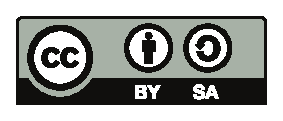
\includegraphics[width=2cm]{by-sa-corr.eps}
\end{flushright}

\Header{Тестирование программ}

Тестирование программ, т.е. проверка уже написанной программы на наличие ошибок в них и поиск этих ошибок "--- 
это один из важнейших навыков программиста"=олимпиадника. 
Я бы сказал, что он важнее любого конкретного отдельно взятого алгоритма, а то и группы алгоритмов.

В классических школьных олимпиадах вы весь тур решаете задачи, а проверяются они только после тура. 
(Или во время тура, но вам не сообщают результаты проверки "--- или сообщают, но только на тестах из условия "--- это все не очень существенно отличается.) 
В результате, если ваша программа не пройдет часть тестов жюри, вы никак не сможете это исправить. 
Поэтому на классических олимпиадах тестирование "--- не просто важный, а сверхважный навык.

На современных школьных олимпиадах высокого уровня "--- на международной, всероссийской олимпиадах; также есть слухи (на сентябрь 2014 г.), 
что эта система может быть распространена на региональные (областные) олимпиады, "--- применяется система с <<токенами>>, 
в которой участники могут проверить свое решение на полном наборе тестов во время тура олимпиады.
На такую проверку налагаются определенные ограничения, но тем не менее это, конечно, существенно снижает важность умения тестировать.
Тем не менее все равно навык тестирования остается важным; умея быстро найти тест, на котором ваша программа не работает, вы сможете все ошибки
и исправить быстрее.

В олимпиадах, проводимых по стандарту ACM (это в первую очередь командные олимпиады), участники тоже могут сдавать решения на проверку на полном наборе тестов по ходу тура, но за каждую неудачную попытку начисляются штрафные минуты. 
В дополнение к этому, если решение не проходит хотя бы один тест, оно не засчитывается вообще. 
В результате умение быстро и надежно тестировать здесь также является весьма существенным.

Итак, тестировать нужно уметь и уметь хорошо.

Когда вы решаете задачи "--- не важно, где "--- на учебных занятиях, на олимпиаде или еще где"=либо "--- всегда старайтесь все задачи решать с минимальным числом штрафных попыток. Старайтесь все свои решения проверять максимально тщательно, и воспринимайте любую неудачную попытку как показатель того, что тестируете вы все"=таки неидеально. Радуйтесь всегда, когда сложная задача проходит все тесты с первой попытки, и огорчайтесь, если нет "--- даже если никаких штрафов за неверную попытку не предусмотрено.

Поэтому в этой теме мы обсудим, как же надо тестировать.

\header{Стратегия тестирования}
Конечно, необходимость тестирования и необходимый объем сильно зависят от сложности задачи. 
Если вы пишите задачу, которая для вас очевидно является очень простой, и вы абсолютно уверены, что напишите ее без ошибок, 
то ее скорее всего можно и не очень тщательно тестировать. 
Часто бывает достаточно просто прогнать тест из условия и еще пару тестов "--- и можно сдавать. 
Особенно это относится к ситуации, когда время ценно, а штраф за ошибочную попытку отсутствует "--- как в системе с токенами.

Аналогично, если до конца тура остается пара минут, то вы просто не успеете провести полный цикл тестирования. 
Но если задача не совсем элементарна, или если цена ошибки высока, то тестируйте задачу тщательно. Ни в коем случае не пренебрегайте этим; 
лучше вы потратите лишнее время на тестирование, но не получите штрафа и будете уверены, что задача работает.

\header{Какие тесты надо использовать}
Главное правило тестирования следующее:

\begin{framed}
Тестирование "--- это последовательный, систематический процесс.
\end{framed}

Вы не должны тестировать задачу по принципу <<подсуну несколько случайных тестов и посмотрю, разумные ли результаты выдает программа>>. 
Не следует придумывать какие попало тесты, не следует стараться понаворотить в один тест побольше всего интересного. 
Вместо этого надо четко понимать, зачем вы делаете каждый очередной тест, понимать, какие тесты вы будете использовать дальше, и так далее.

Соображения, которые я излагаю ниже, конечно, применимы не к каждой задаче "--- но в каждой задаче смотрите, что из того, что указано ниже, применимо.

\lheader{Минимальные тесты} 
Первым делом подсуньте своей программу \textit{самый маленький тест}, какой только возможен. Это зачастую $N=1$ или даже $N=0$ или что-нибудь подобное. Часто бывает, что такой <<самый маленький>> тест вообще один в своем роде "--- например, существует только одна перестановка из 1 числа, или только один граф без петель с 1 вершиной. Если же нет "--- выберите любой из самых маленьких тестов. Можно даже попробовать два самых маленьких теста; например, если на вход подается массив из $N$ чисел, то попробуйте два теста с $N=1$: когда в массиве единственный элемент равен 1 и когда он равен, например, 137. (А вообще, см. ниже про разнообразие тестов "--- может быть, стоит проверить еще и элемент, равный 0, -1 и -137.) Правда, в этом случае сначала убедитесь, что минимальным тестом не является вообще тест с $N=0$!

(Вообще, многие любят начинать тестирование с теста из условия. На мой взгляд, в большинстве случаев это неправильный подход, почему "--- см. ниже.)

(Однажды ко мне обратился один школьник со словами, что его программа не работает в тестирующей системе, но у него она работает.
Насколько я помню, там вводилось поле $N\times M$ из чисел. 
Я начал тестировать его задачу, введя сначала минимальный тест "--- $N=M=1$, на поле одна единичка. 
Программа зависла.)

После этого чуть увеличьте размер теста (возьмите $N=2$) и постарайтесь протестировать все возможные (!) такие тесты. 
Например, если у вас задана перестановка, проверьте обе возможные перестановки; если граф без петель "--- то все возможные графы с двумя вершинами. 
Как правило, таких тестов не так уж и много, и проверить все не составляет проблем. 
Если же таких тестов бесконечно много, то постарайтесь проверить хотя бы все возможные категории таких тестов. 
Например, в задаче сортировки массива обязательно проверьте случай, когда первое число больше второго, когда оно равно второму и когда оно меньше второго. 
(Это все при $N=2$!) Таких <<категорий>> обычно не так уж и много.

Далее переходите к следующему размеру теста и опять"=таки постарайтесь проверить все возможные тесты или хотя бы все категории тестов. И так далее "--- до тех пор, пока при очередном размере тестов количество возможных тестов или категорий не станет уж очень велико (ну, грубо говоря, больше чем 5--7); часто это бывает уже при $N=3$. В таком случае на этом $N$ проверьте несколько тестов из существенно различных категорий, после чего уже плавно переходите к следущему разделу.

\lheader{Простые маленькие тесты}
Далее попробуйте несколько небольших тестов. Как правило, сюда же попадет тест из условия. 
Старайтесь эти тесты делать различными, добавляя в них те или иные <<фичи>>, которые могут оказаться важны, 
но которые вы толком не смогли протестировать раньше из-за того, что тесты были маленькие. 
Например, это могут быть мосты или циклы в графе, несвязные графы с ненулевым количеством ребер в каждой компоненте связности, 
или сложные "--- сначала возрастающие, потом убывающие, потом опять возрастающие перестановки типа 3 4 1 2, или массивы, в которые есть одинаковые числа, 
но они не соседние (2 1 3 2) и т.п.

\lheader{<<Подлые>> тесты}
Подумайте, какие в вашей задаче могут быть <<подлые>> тесты. 
Например, когда решения нет, или когда решение в каком-то смысле пограничное, или не такое, как во многих тестах и т.п.
Если у вас есть в программе особые случаи, то подумайте и о них. 
Протестируйте все такие тесты, при этом старайтесь на каждый случай придумывать не очень большой пример. 
(Не обязательно совсем минимальный, но и не надо лишних наворотов.)

\lheader{Пороговые тесты}
Часть бывает так, что в вашей задаче есть тесты, где при небольшом изменении входные данных ответ "--- или по крайней мере логика его получения "--- меняются сильно.
Например, задача <<выведите наибольшую степень двойки, которая меньше данного числа $N$>>. 
Ясно, что таким пороговым случаем является случай, когда $N$ само является степенью двойки. 
Например, на всем отрезке $[32,63]$ ответ один и тот же, а вот когда $N$ становится равно 64, ответ резко меняется.
Или, например, в вашей задаче есть ровно два <<пути>>, и вам нужно выбрать минимальный "--- тогда пороговой оказывается ситуация,
когда оба пути имеют одинкаовую длину: тут при вариации входных данных минимальным будет становиться то один путь, то другой.

Обязательно протестируйте такие тесты, причем не только сам пороговый тест, но и $\pm 1$ от него, а то и $\pm 2$. 
Например, в задаче про степень двойки обязательно протестируйте числа 63, 64, 65, а может быть, еще и 62 и 66 "--- 
чтобы убедиться, что переход на новый ответ или вариант его получения происходит в правильный момент.


Разнообразие

Не по формату, но по смыслу

Почему не тест из условия


\inputanswers

\end{document}
